\documentclass[a4]{beamer}
\usepackage{amssymb}
\usepackage{graphicx}
\usepackage{subfigure}
\usepackage{newlfont}
\usepackage{amsmath,amsthm,amsfonts}
%\usepackage{beamerthemesplit}
\usepackage{pgf,pgfarrows,pgfnodes,pgfautomata,pgfheaps,pgfshade}
\usepackage{mathptmx}  % Font Family
\usepackage{helvet}   % Font Family
\usepackage{color}


\setbeamercovered{dynamic}

\title[MA4704]{Technology Mathematics 4 (Statistics) \\ {\normalsize MA4704 Lecture 4A}}
\author[Kevin O'Brien]{Kevin O'Brien \\ {\scriptsize Kevin.obrien@ul.ie}}
\date{Spring Semester 2013}
\institute[Maths \& Stats]{Dept. of Mathematics \& Statistics, \\ University \textit{of} Limerick}

\renewcommand{\arraystretch}{1.5}

\begin{document}

\begin{frame}
\titlepage
\end{frame}
%---------------------------------------------------------------------%
\frame{
\frametitle{Binomial Expected Value and Variance}
\begin{itemize}
\item Lecture is called off for Thursday of Week 4.
\item The first midterm is to take place Thursday of Week 5.
\item The first midterm will cover:
\begin{itemize}
\item Basic Probability
\item Descriptive statistics (mean, median variance etc)
\item Discrete probability distributions (binomial and Poisson)
\item The exponential distribution
\item (The normal distribution will be not be included).
\end{itemize}
\end{itemize}
}
%------------------------------------------------------------------%
\frame{
\frametitle{Binomial Expected Value and Variance}


If the random variable X has a binomial distribution with parameters n
and p, we write
\[ X \sim B(n,p) \]

Expectation and Variance
If $X \sim B(n,p)$, then:

\begin{itemize}
\item Expected Value of X : E(X) = np
\item Variance of X : Var(X) = np(1-p)
\end{itemize}
}
%---------------------------------------------------------------------%
\begin{frame}
\frametitle{Binomial Distribution: Example 1}
\begin{itemize} \item Diagrams of the probability mass functions of the two binomial
distributions $B(10, 0.5)$ and $B(10, 0.25)$ are shown in the bar-plots (next slide). \item Which
is which? Give a reason for your answer.
\end{itemize}
\end{frame}
%---------------------------------------------------------------------%
\begin{frame}
\frametitle{Binomial Distribution}
\begin{figure}
  % Requires \usepackage{graphicx}
  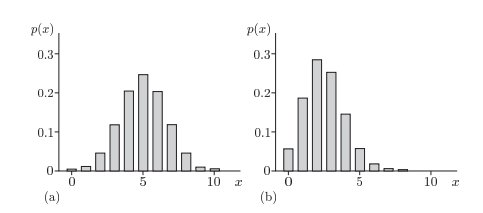
\includegraphics[scale=0.60]{4ABarCharts.jpg}\\
  \caption{Bar Charts}
\end{figure}
\end{frame}
%---------------------------------------------------------------------%
%---------------------------------------------------------------------%
\begin{frame}
\frametitle{Binomial Distribution: Example 1}
\begin{itemize}
\item Clearly. Figure A is $B(10, 0.5)$ and Figure B is $B(10, 0.25)$.
\item The mean of B(10, 0.5) is 5, and the mean of B(10, 0.25) is 2.5. These values correspond to the apex of both distributions on the previous slide.
\item Also the variance of a binomial distribution corresponding to $B(10, 0.25)$ is $1.875$, while for $B(10, 0.25)$ it is $2.500$.
\item A visual inspection of the two bar-charts would indicate that Figure A has the higher variance.
\end{itemize}
\end{frame}
%---------------------------------------------------------------------%
\begin{frame}
\frametitle{Binomial Distribution: Example 2}

\begin{itemize}
\item Components are placed into containers containing 100 items.
\item After an inspection of a large number of containers the average number of defective items was found to be 10 with a standard deviation of three.
\item Is the binomial distribution a good useful distribution, given the observed data?
\end{itemize}
\end{frame}
%---------------------------------------------------------------------%
\begin{frame}
\frametitle{Binomial Distribution: Example 2}

\begin{itemize}
\item Let the number of containers be the number of independent trials is $n=100$.
\item A success may be defined as a defective component.
\item The probability of a success is approximate $p=0.10$. (The probability of ``failure" is $1-p=0.9$).
\item The expected number of defective components is $np=10$, which concurs with our observed data.
\item The variance is computed as \[np(1-p) = 100 \times 0.1 \times 0.9 = 9\]
\item The observed standard deviation is 3 units, i.e. a variance of 9 square units.
\item Yes the binomial distribution is useful in this case.
\end{itemize}
\end{frame}
%------------------------------------------------------------------%
\frame{
\frametitle{Poisson Expected Value and Variance}


If the random variable X has a Poisson distribution with parameter $m$, we write
\[ X \sim Poisson(m) \]


\begin{itemize}
\item Expected Value of X : E(X) = m
\item Variance of X : $Var(X) = m$
\item Standard Deviation of X : $SD(X) = \sqrt{m}$
\end{itemize}
}
%------------------------------------------------------------------%
\frame{
\frametitle{Poisson Distribution : Example} 

\begin{itemize}
\item The number of faults in a fibre optic cable were recorded for each kilometre length of cable.
\item The mean number of faults was found to be 4 faults per kilometre.
\item The standard deviation of the number of faults was found to be 2 faults per kilometre.
\item Is the Poisson Distribution is a useful technique for modelling the number of faults in fibre optic cable?
\item (Looking at the last slide, the answer is yes).
\end{itemize}

}
%---------------------------------------------------------------------%
\begin{frame}
\frametitle{Poisson Approximation of the Binomial}
\begin{itemize}
\item The Poisson distribution can sometimes be used to approximate the
binomial distribution
\item When the number of observations n is large, and the success probability
p is small, the $B(n,p)$ distribution approaches the Poisson distribution
with the parameter given by $m = np$.
\item This is useful since the computations involved in calculating binomial
probabilities are greatly reduced.
\item As a rule of thumb, n should be greater than 50 with p very small, such
that np should be less than 5.
\item If the value of p is very high, the definition of what constitutes a
``success" or ``failure" can be switched.
\end{itemize}
\end{frame}

%---------------------------------------------------------------------%
\begin{frame}
\frametitle{Poisson Approximation: Example}

\begin{itemize}
\item Suppose we sample 1000 items from a production line that is producing, on
average, $0.1\%$ defective components.
\item Using the binomial distribution, the probability of exactly 3 defective items in
our sample is
\[P(X = 3) = ^{1000}C_{3} \times 0.001^{3} \times 0.999^{997}\]
\end{itemize}
\end{frame}

%---------------------------------------------------------------------%
\begin{frame}
\frametitle{Poisson Approximation: Example}
Lets compute each of the component terms individually.

\begin{itemize}
\item $^{1000}C_{3}$
\[^{1000}C_{3} = \frac{1000 \times 999 \times 998}{3 \times 2 \times 1} = 166,167,000\]
\item $0.001^3$
\[0.001^3 = 0.000000001\]
\item $0.999^{997}$
\[0.999^{997} = 0.36880\]
\end{itemize}


Multiply these three values to compute the binomial probability
$P(X = 3) = 0.06128$
\end{frame}

\begin{frame}
\frametitle{Poisson Approximation: Example}
\begin{itemize}
\item Lets use the Poisson distribution to approximate a solution.
\item First check that $n \geq 50$ and $np < 5$ (Yes to both).
\item We choose as our parameter value $m = np = 1000 \times 0.001 = 1$
\end{itemize}
\[P(X = 3) = \frac{e^{-1} \times 1^3}{3!} = \frac{e^{-1}}{6} = \frac{0.36787}{6} = 0.06131 \]
Compare this answer with the Binomial probability
P(X = 3) = 0.06128.
Very good approximation, with much less computation effort.
\end{frame}


\end{document} 
